\chapter{AutoMISC}
\label{app:automisc}


\Cref{fig:automisc} shows a system flow diagram of AutoMISC. First, each volley (turn of speech) is parsed into one or more utterances (units of thought) by the Parser module. Then, utterance-level annotations, i.e. behavioural codes, are assigned by the Annotator module to each utterance. Up to $k=5$ prior volleys are included in the Annotator module when coding utterances.



\section*{AutoMISC Validation}
\label{appendix:automisc_val}


We present the pairwise Cohen's $\kappa$ values, for both counsellor and client codes, in \Cref{fig:ck}. All $\kappa$ values fall between 0.55-0.81, indicating moderate to substantial agreement between each pair of raters beyond chance~\cite{cohenrange}. The Cohen's $\kappa$ values between AutoMISC and the expert annotators (Annotators 1 and 2) were \textbf{0.63} and \textbf{0.58} for counsellor codes, and \textbf{0.63} and \textbf{0.69} for client codes, respectively.

\section*{Statistical Validation of Inter-Rater Reliability}
To estimate how these reliability findings generalize to more transcripts, we computed the \textbf{asymptotic variance} of Fleiss' $\kappa$ to calculate two-tailed $p$-values. For both counsellor and client codes, the asymptotic variance was on the order of $10^{-6}$, resulting in $p$-values of $p<.001$. These extremely low $p$-values indicate that the inter-rater agreement is highly statistically significant beyond chance. A post-hoc power analysis confirmed that our study was highly powered (estimated power: 1.00) to detect nonzero agreement, i.e., there is a near-certain probability to detect significant inter-rater reliability.

\begin{figure*}[!ht]
	\centering
	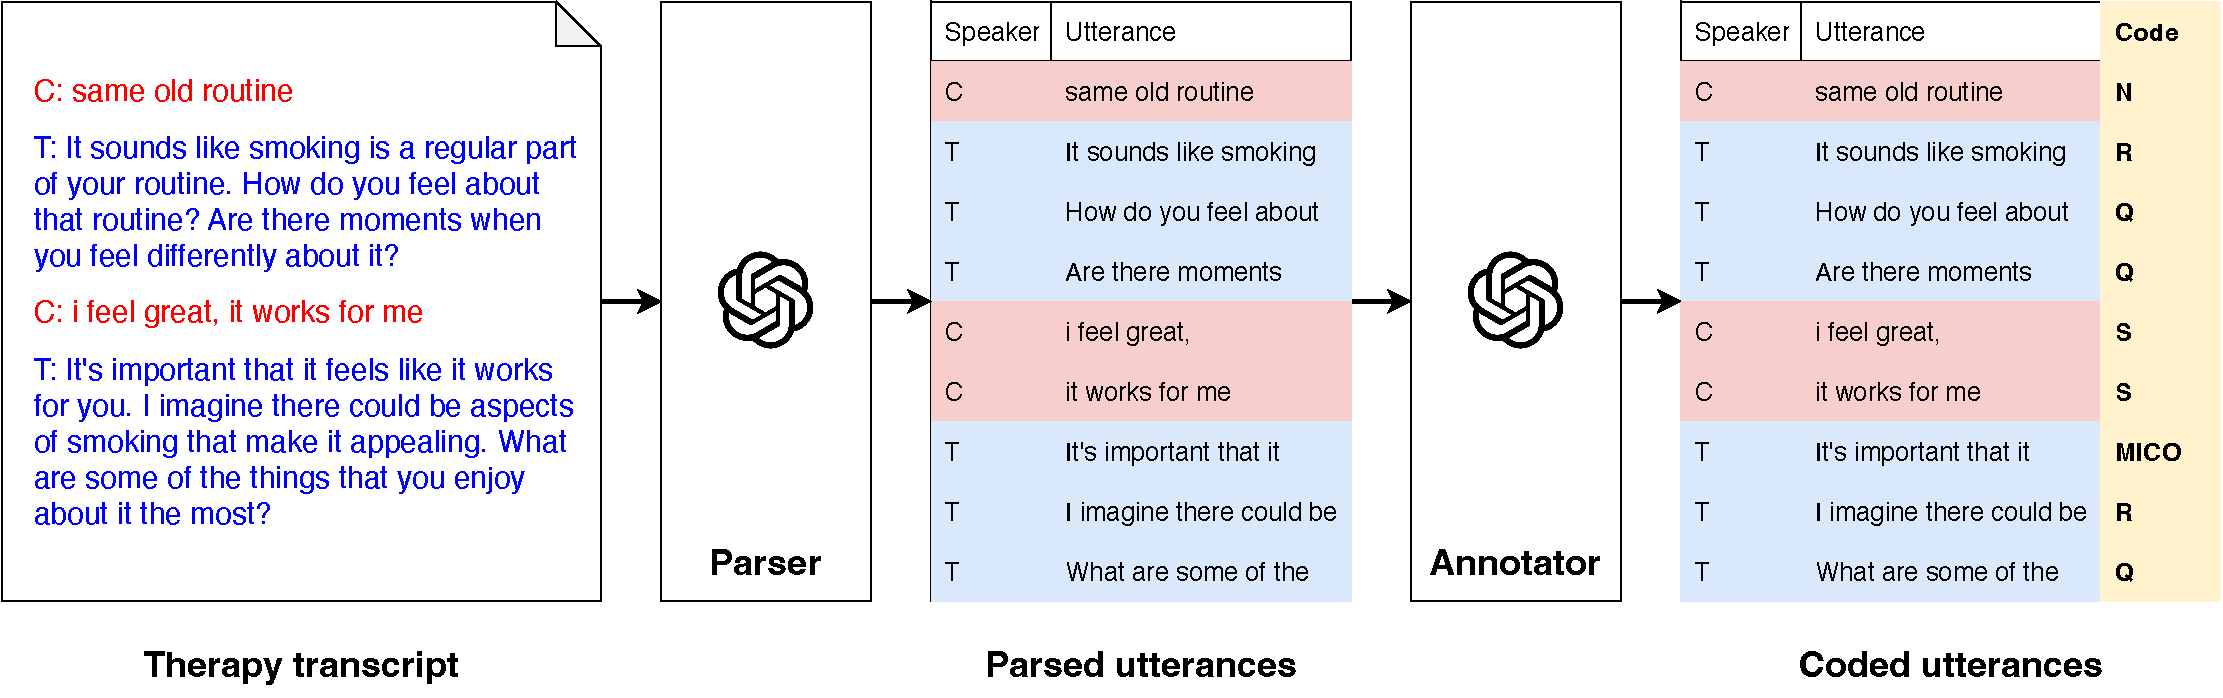
\includegraphics[width=\linewidth]{fig/automisc.pdf}
	\caption[AutoMISC system diagram]{AutoMISC system diagram.}
	\label{fig:automisc}
\end{figure*}

\begin{figure*}[!ht]
	\centering
	\begin{subfigure}[b]{0.48\textwidth}
		\centering
		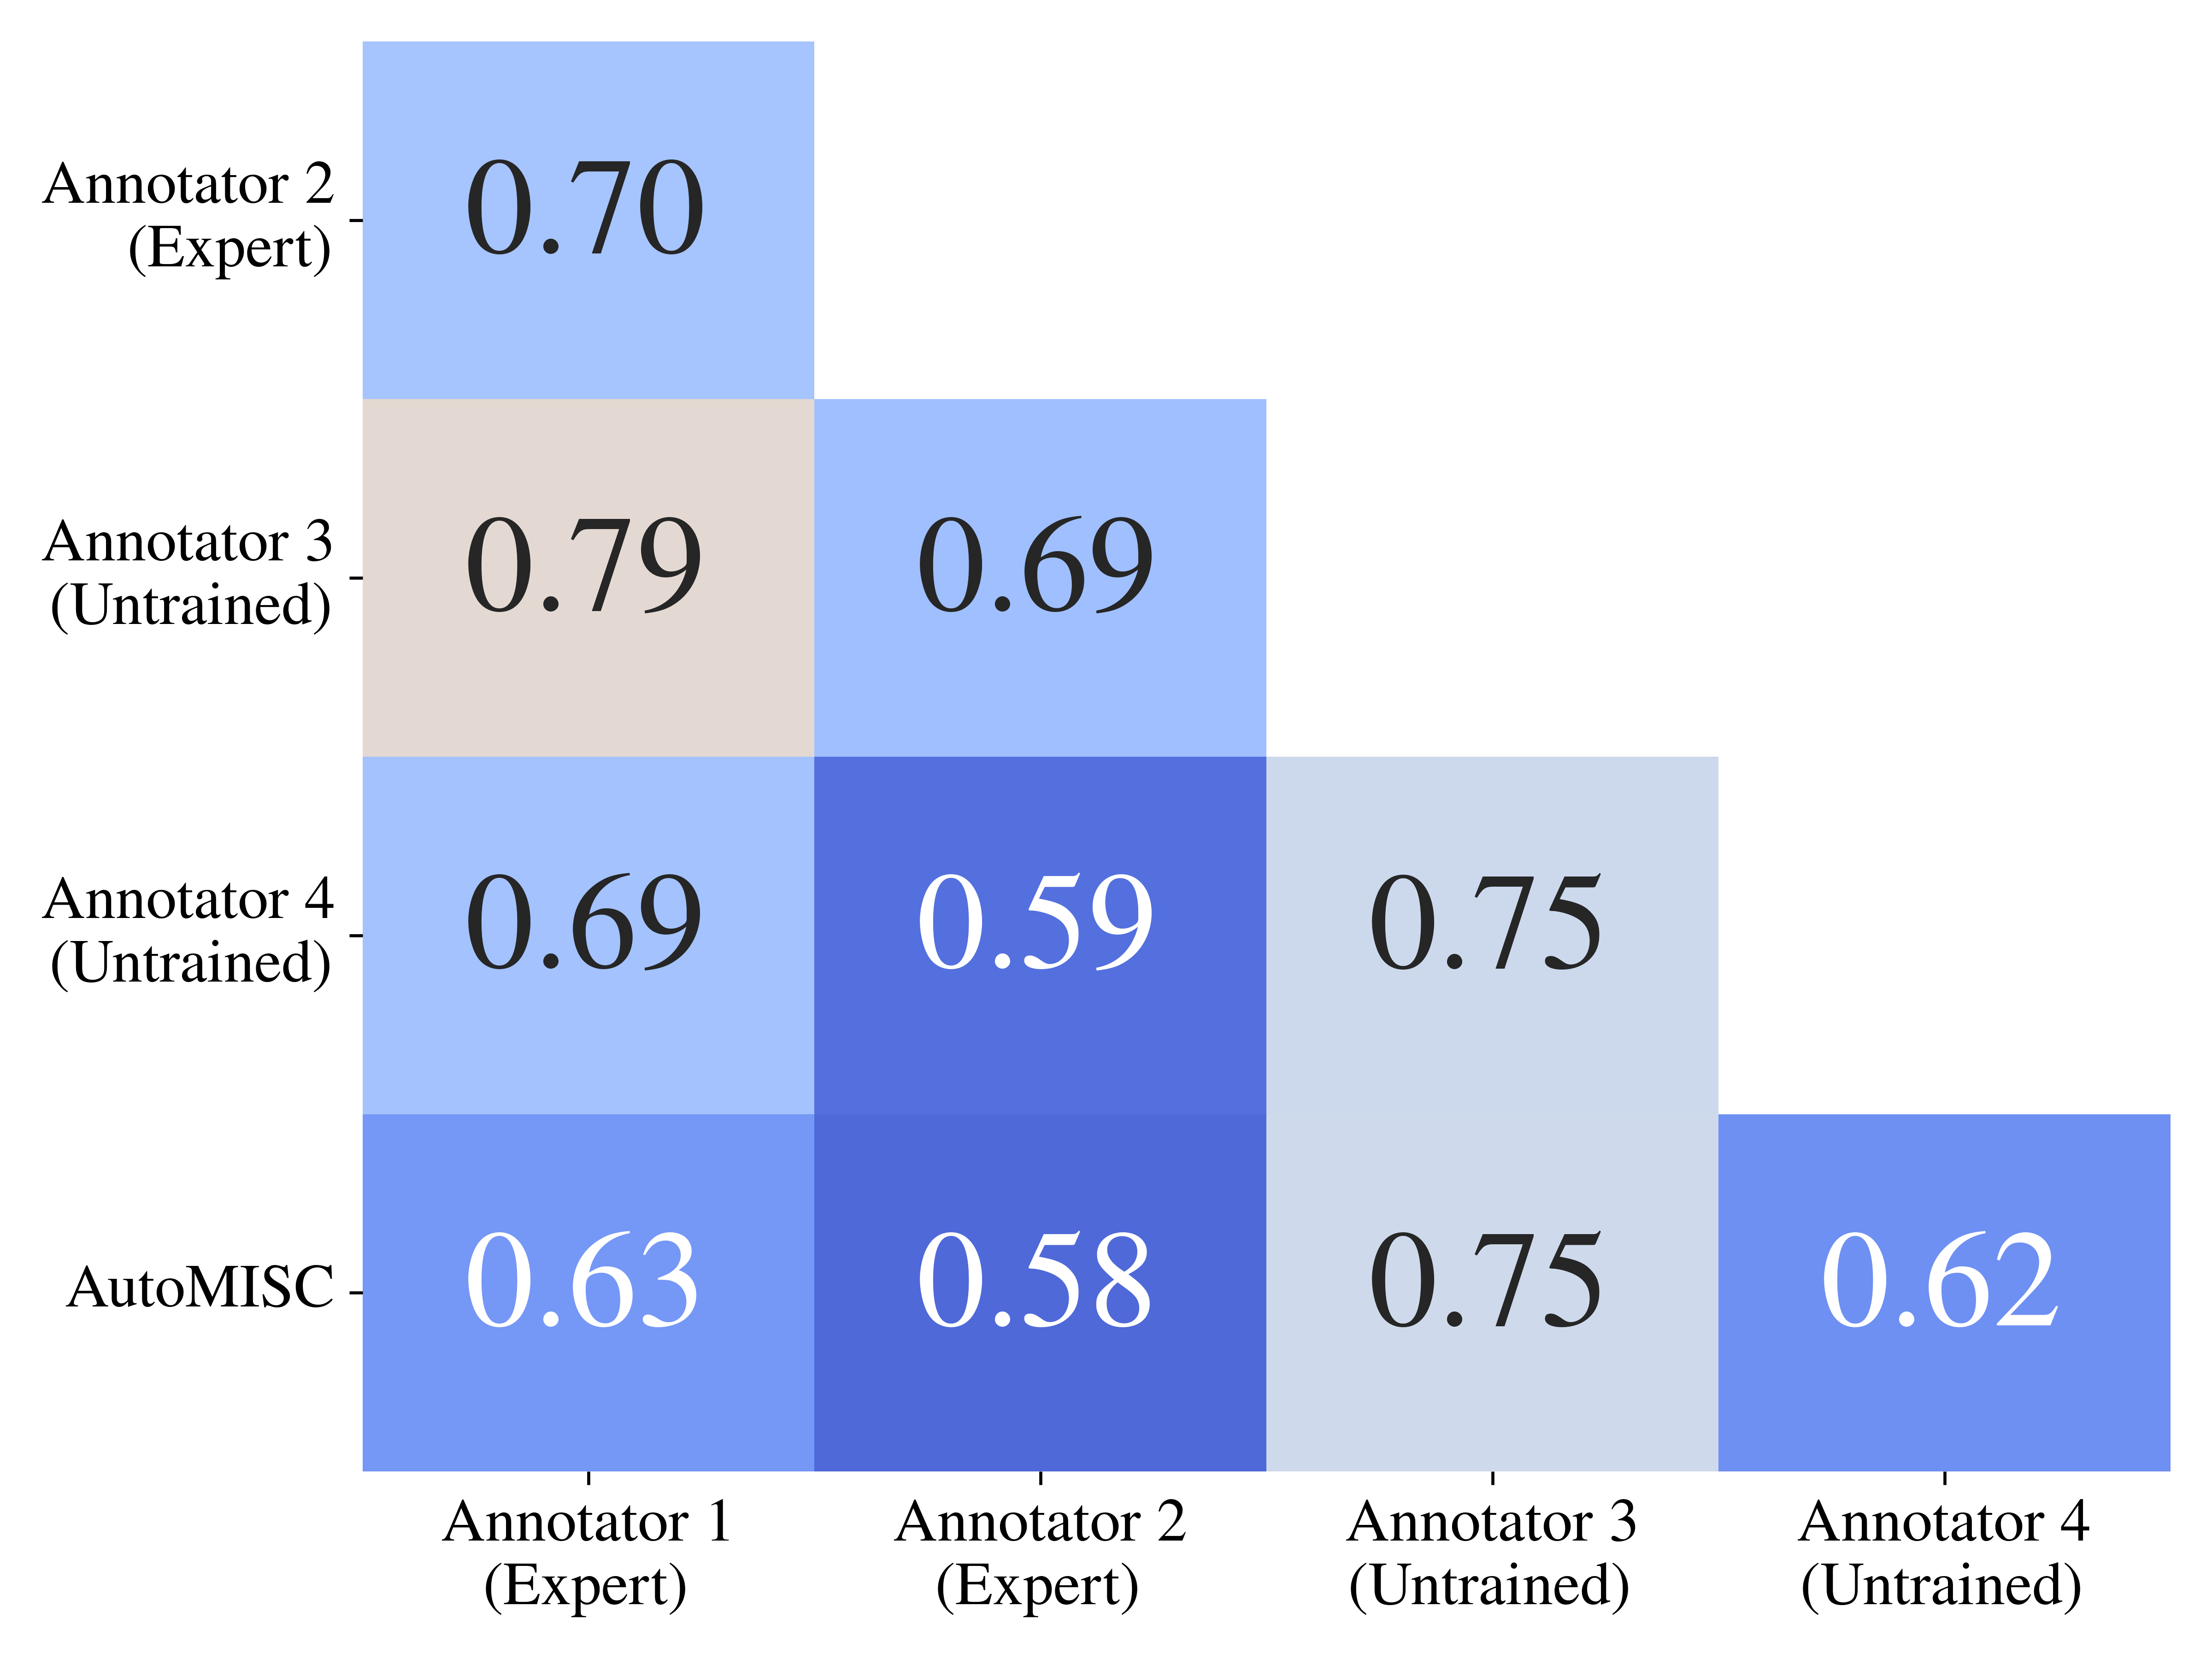
\includegraphics[width=\textwidth]{fig/co_kappa.png}
		\caption{Counsellor codes}
		\label{fig:co_k}
	\end{subfigure}
	\hfill
	\begin{subfigure}[b]{0.48\textwidth}
		\centering
		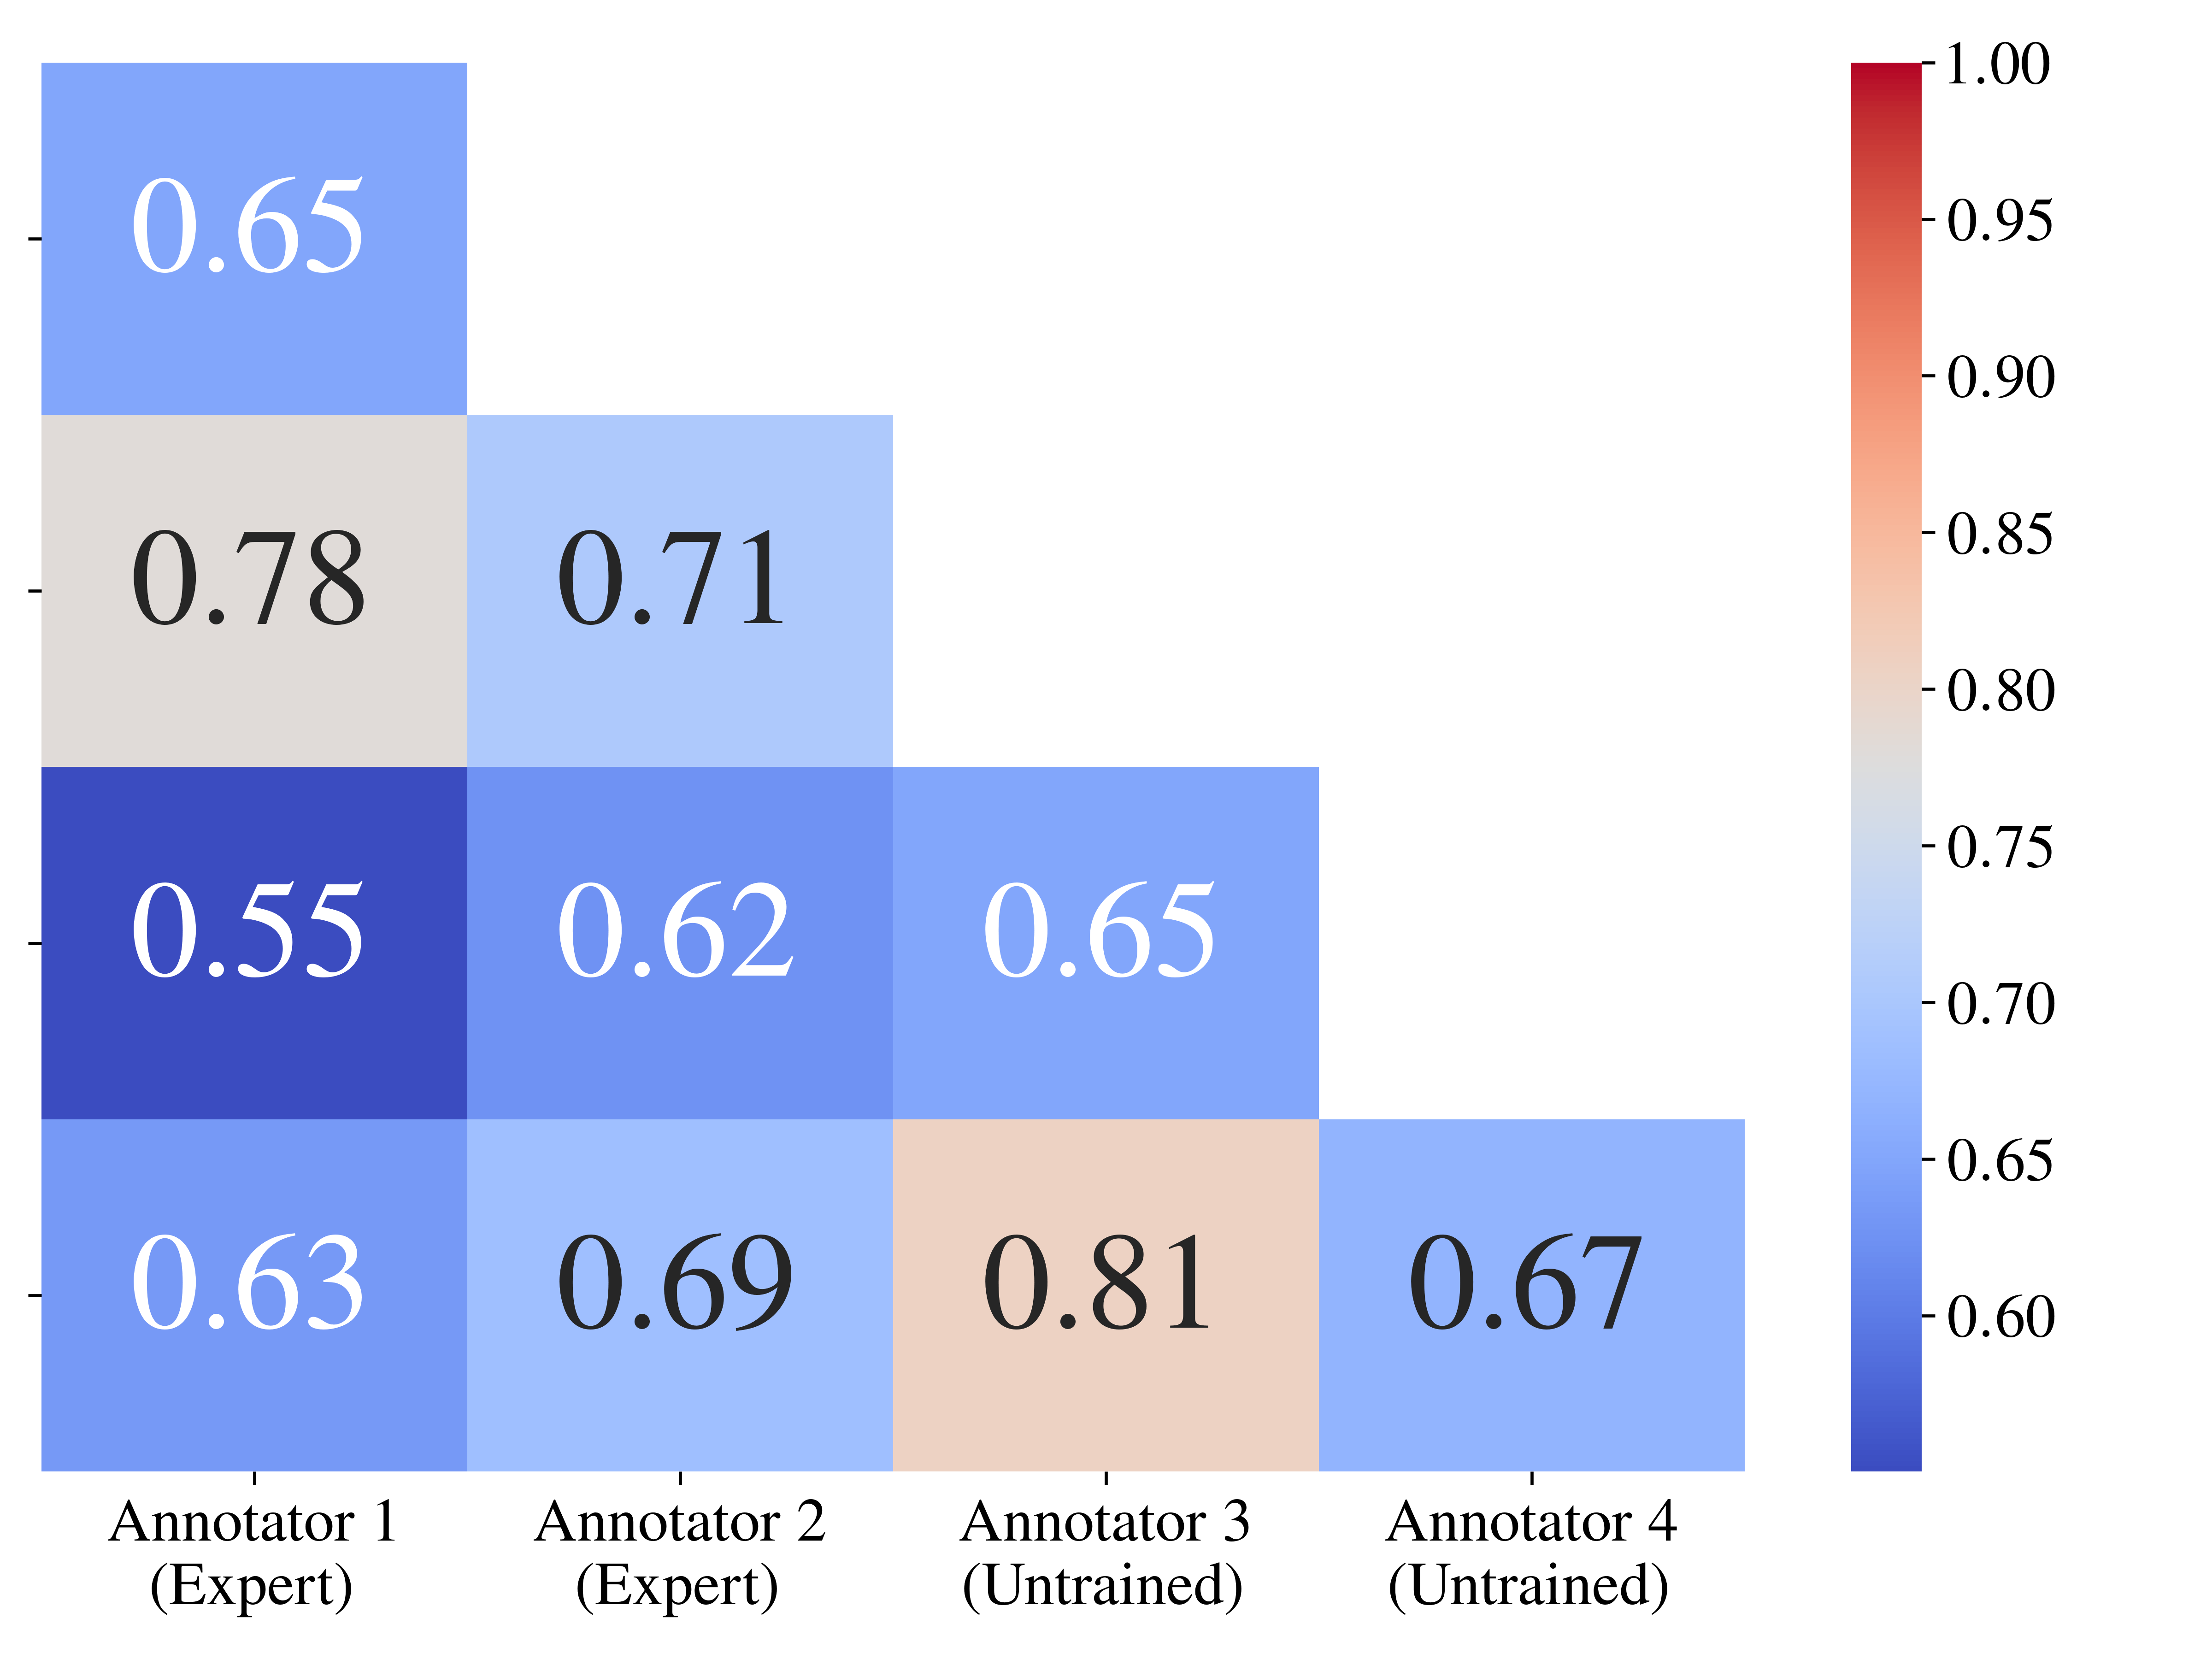
\includegraphics[width=\textwidth]{fig/cl_kappa.png}
		\caption{Client codes}
		\label{fig:cl_k}
	\end{subfigure}
	\caption[Cohen's $\kappa$ between rater pairs on behaviour code annotations]{Cohen's $\kappa$ between rater pairs on behaviour code annotations.}
	\label{fig:ck}
\end{figure*}





\section*{AutoMISC System Prompts}
\label{appendix:automisc_prompts}



\begin{tcolorbox}[
		breakable,
		colback=magenta!5!blue!10,        % Subtle pink/purple background
		colframe=magenta!60!blue!40,      % Darker purple/pink frame
		fontupper=\small,
		title=\subsection*{Parser Prompt}
	]

	You are a highly accurate Motivational Interviewing (MI) counselling session annotator.
	Your task is to segment the given volley into utterances.\\

	Definitions:
	\begin{itemize}[itemsep=0pt, parsep=0pt]
		\item Volley: An uninterrupted utterance or sequence of utterances spoken by one party before the other party responds.
		\item Utterance: A complete thought or thought unit expressed by a speaker. This could be a single sentence, phrase, or even a word if it conveys a standalone idea. Multiple utterances often run together without interruption in a volley.
	\end{itemize}

	Output Format:
	\begin{itemize}[itemsep=0pt, parsep=0pt]
		\item Return the segmented utterances as a Python list of strings.
	\end{itemize}

	Examples:
	Below are examples of how to segment a volley into utterances. Follow this structure when processing new inputs.

	\lstset{
		basicstyle=\ttfamily\small,
		breaklines=true,
		frame=single,
		backgroundcolor=\color{gray!10}
	}
	\begin{lstlisting}
Input:  "Why haven't you quit smoking? Are you ever going to quit?"
Output: ["Why haven't you quit smoking?", "Are you ever going to quit?"]

Input:  "How long since your last drink? Do you feel ok?"
Output: ["How long since your last drink?", "Do you feel ok?"]

Input:  "I can't quit. I just can't do it. I don't have what it takes. I just cannot stop."
Output: ["I can't quit.", "I just can't do it.", "I don't have what it takes.", "I just cannot stop."]

Input:  "I don't want to go to the bars every day. I don't want my kids to see that. I want my kids to have a better life than that."
Output: ["I don't want to go to the bars every day.", "I don't want my kids to see that.", "I want my kids to have a better life than that."]
\end{lstlisting}

\end{tcolorbox}



\begin{tcolorbox}[breakable,
		% width=\textwidth, % Full page width
		colback=magenta!5!blue!10,        % Subtle pink/purple background
		colframe=magenta!60!blue!40,      % Darker purple/pink frame
		fonttitle=\bfseries, % Bold title font
		fontupper=\small,
		title=\subsection*{Counsellor Utterance Classification Prompt}]

	You are a highly accurate Motivational Interviewing (MI) counselling session annotator.
	Your task is to analyze an excerpt from a counselling session of up to five volleys and categorize the counsellor's final utterance.\\

	Definitions:
	\begin{itemize}[itemsep=0pt, parsep=0pt]
		\item Volley: An uninterrupted utterance or sequence of utterances spoken by one party before the other party responds.
		\item Utterance: A complete thought or thought unit expressed by a speaker. This could be a single sentence, phrase, or even a word if it conveys a standalone idea. Multiple utterances often run together without interruption in a volley.
	\end{itemize}

	Task:
	\begin{enumerate}[itemsep=0pt, parsep=0pt]
		\item Determine whether the counsellor's final utterance in the excerpt belongs to one of the following categories:
		      \begin{itemize}[itemsep=0pt, parsep=0pt]
			      \item MI-Consistent (MICO): Directly prescribed in Motivational Interviewing (excluding Reflections and Questions).
			      \item MI-Inconsistent (MIIN): Directly proscribed in Motivational Interviewing principles.
			      \item Reflection or Question (RQ): Includes Reflections or Questions.
			      \item Other (Other): Does not fit the above categories.
		      \end{itemize}
		\item Return your analysis as:
		      \begin{itemize}
			      \item explanation: Briefly justify your choice in one to two sentences.
			      \item label: Provide only MICO, MIIN, RQ, or Other.
		      \end{itemize}
	\end{enumerate}

	Behavioural Code Guide:\\

	MI-Consistent (MICO):
	\begin{itemize}[itemsep=0pt, parsep=0pt]
		\item Affirm (AF): Communicates something positive or complimentary about the client's strengths or efforts.
		\item Advise with permission (ADP): After receiving permission, gives advice, makes a suggestion, or offers a solution or possible action.
		\item Emphasize control (EC): Acknowledges, honors, or emphasizes the client's autonomy and freedom of choice.
		\item Raise concern with permission (RCP): After getting permission, points out a possible problem with a client's goal, plan, or intention. Always phrased as the counsellor's concern.
		\item Support (SU): Sympathetic, compassionate, or understanding comments, which agree or side with the client.
	\end{itemize}

	MI-Inconsistent (MIIN):
	\begin{itemize}[itemsep=0pt, parsep=0pt]
		\item Advise without permission (ADWP): Offers suggestions or guidance without asking or receiving permission.
		\item Confront (CON): Directly disagrees, argues, corrects, shames, blames, seeks to persuade, criticizes, judges, labels, moralizes, ridicules, or questions the client's honesty.
		\item Direct (DIR): Gives an order, command, or direction. The language is imperative.
		\item Raise concern without permission (RCWP): Without getting permission, points out a possible problem with a client's goal, plan, or intention.
		\item Warn (WA): Provides a warning or threat, implying negative consequences unless the client takes a certain action.
	\end{itemize}

	Reflection or Question (RQ):
	\begin{itemize}[itemsep=0pt, parsep=0pt]
		\item Question (Q): Asks a question to gather information, understand, or elicit the client's story.
		\item Reflection (R): Makes a statement that reflects back content or meaning previously offered by the client, usually (but not always) in the client's immediately preceding utterance.
	\end{itemize}

	Other (Other):
	\begin{itemize}[itemsep=0pt, parsep=0pt]
		\item Facilitate (FA): Simple utterance that functions as a ``keep-going'' acknowledgment, e.g., ``Mm-hmm'', ``I see'', ``Go on''.
		\item Filler (FI): Pleasantries such as ``Good morning'', ``Nice weather we're having'', etc.
		\item Giving Information (GI): Provides information to the client, explains something, educates or provides feedback, or discloses personal information.
		\item Structure (ST): Gives information about what will happen directly to the client throughout the course of treatment or within a study format, in this or subsequent sessions.
	\end{itemize}

	Based on the following excerpt, determine which category the counsellor's last utterance falls into and respond accordingly. After you're done, go back over the RQ category and assign a subcategory of ``R'' for reflection or ``Q'' for question.
\end{tcolorbox}



\begin{tcolorbox}[breakable,
		% width=\textwidth, % Full page width
		colback=magenta!5!blue!10,        % Subtle pink/purple background
		colframe=magenta!60!blue!40,      % Darker purple/pink frame
		fonttitle=\bfseries, % Bold title font
		fontupper=\small,
		title=\subsection*{Client Utterance Classification Prompt}]

	You are a highly accurate Motivational Interviewing (MI) counselling session annotator.
	Your task is to analyze an excerpt from a counselling session of up to five volleys and categorize the client's final utterance.
	The target behaviour change of this conversation is smoking cessation.

	Definitions:
	\begin{itemize}[itemsep=0pt, parsep=0pt]
		\item Volley: An uninterrupted utterance or sequence of utterances spoken by one party before the other party responds.
		\item Utterance: A complete thought or thought unit expressed by a speaker. This could be a single sentence, phrase, or even a word if it conveys a standalone idea. Multiple utterances often run together without interruption in a volley.
	\end{itemize}

	Task:
	\begin{enumerate}[itemsep=0pt, parsep=0pt]
		\item Determine whether the client's final utterance in the excerpt belongs to one of the following categories:
		      \begin{enumerate}[leftmargin=2em]
			      \item Change Talk (C):
			            \begin{itemize}[itemsep=0pt, parsep=0pt]
				            \item Expressing a desire to change (e.g., ``I really want to quit smoking'').
				            \item Recognizing the downsides of the current behavior (e.g., ``My health is suffering because I smoke'').
				            \item Identifying potential benefits of making a change (e.g., ``I would feel better if I exercised more'').
				            \item Demonstrating commitment to change (e.g., ``I'm ready to make a plan to lose weight'').
			            \end{itemize}

			      \item Sustain Talk (S):
			            \begin{itemize}[itemsep=0pt, parsep=0pt]
				            \item Minimizing the problem (e.g., ``It's not that bad, I can handle it'').
				            \item Highlighting difficulties or challenges of change (e.g., ``I don't know if I can give up smoking'').
				            \item Expressing doubts about the ability to change (e.g., ``I've tried to quit before and failed'').
				            \item Focusing on the positive aspects of the current behavior (e.g., ``Smoking helps me relax'').
			            \end{itemize}

			      \item Neutral Talk (N):
			            \begin{itemize}[itemsep=0pt, parsep=0pt]
				            \item Describing current situations or circumstances without expressing a strong pro- or anti-change stance (e.g., ``I've been thinking about making changes'').
				            \item Asking questions related to the situation or change process (e.g., ``What are the pros and cons of changing?'').
				            \item Making general or factual statements about the issue (e.g., ``It's important to take care of my health'').
			            \end{itemize}
		      \end{enumerate}
		\item Return your analysis as:
		      \begin{itemize}
			      \item explanation: Briefly justify your choice in 1-2 sentences.
			      \item label: Provide only ``C'', ``S'', or ``N''.
		      \end{itemize}
	\end{enumerate}

\end{tcolorbox}
\vspace{1em}
\section*{Demographics of the Annotators}

% \multicollinenumbers
As described in \cref{subsec:automisc}, we enlisted four annotators --- two experts and two novices --- to annotate 10 of the 106 transcripts (comprising 821 utterances) from our study. High alignment between the annotators' labels and the AutoMISC annotations serves as an indicator of AutoMISC's validity. Below, we present their demographic information, following the guidelines proposed by \citet{bender-friedman-2018-data}.


\renewcommand{\arraystretch}{1.1} % optional, if you want extra vertical spacing
% \arrayrulecolor{gray!50}         % adjust the shade of grey as desired

\begin{table}[!ht]
	\centering
	\begin{threeparttable}
		\caption{Demographic Information of Annotators}
		\label{tab:annotator-demographics}
		\begin{tabular}{%
			@{}p{0.25\textwidth}
			p{0.15\textwidth}
			p{0.15\textwidth}
			p{0.15\textwidth}
			p{0.15\textwidth}@{}}
			\toprule
			                                 & \textbf{Annotator \#1\tnote{1}}
			                                 & \textbf{Annotator \#2\tnote{2}}
			                                 & \textbf{Annotator \#3\tnote{3, 4}}
			                                 & \textbf{Annotator \#4\tnote{3, 4}}                                             \\
			\midrule
			\arrayrulecolor{gray!50}
			\textbf{Sex}                     & Female                             & Female    & Male          & Male          \\
			\hline
			\textbf{Age Group (years)}       & 60--69                             & 40-49     & 20-29         & 20-29         \\
			\hline
			\textbf{Race/Ethnicity}          & White                              & White     & Mixed         & Asian         \\
			\hline
			\textbf{Native Language}         & English                            & English   & English       & Mandarin      \\
			\hline
			\textbf{Student Status}          & No                                 & No        & Yes           & Yes           \\
			\hline
			\textbf{Employment Status}       & Full-Time                          & Full-Time & N/A           & N/A           \\
			\hline
			\textbf{Highest Education}       & Graduate                           & Graduate  & Undergraduate & Undergraduate \\
			\hline
			\textbf{Country of Residence}    & Canada                             & Canada    & Canada        & Canada        \\
			\hline
			\textbf{Country of Birth}        & Canada                             & Canada    & Canada        & China         \\
			\hline
			\textbf{Training in Linguistics} & No                                 & No        & No            & No            \\
			\hline
			\textbf{Training in MI}          & Yes                                & Yes       & No            & No            \\
			\arrayrulecolor{black}
			\bottomrule
		\end{tabular}

		\begin{tablenotes}
			\footnotesize
			\item[1]
			Motivational Interviewing Network of Trainers (MINT) member since 2009;
			Motivational Interviewing Treatment Integrity (MITI) coding trained; broad training
			and coaching experience.
			\item[2]
			Introductory-Intermediate-Advance MI training;
			MINT member since 2014;
			MI supervision; MITI training.
			\item[3, 4]
			Engineering graduate student with no formal training in MI.
		\end{tablenotes}

	\end{threeparttable}
\end{table}
